\newpage
\chapter{METODOLOGIA}\label{cap:metodo}
Neste capítulo é apresentado a fundamentação teórica, onde é descrito detalhadamente o método utilizado no desenvolvimento do  trabalho. Em seguida você vai ler 3 parágrafos de Lorem ipsum para encher linguíça.

\lipsum[3-5]



\section{Inserção de Imagens} \label{sec:imagens}
A figura \ref{fig:metodo} apresenta um exemplo de como adicionar uma imagem ao seu trabalho. Em seguida você vai ler 2 parágrafos de Lorem ipsum para encher linguíça.

\lipsum[2-4]


\begin{figure}[H]
\centering
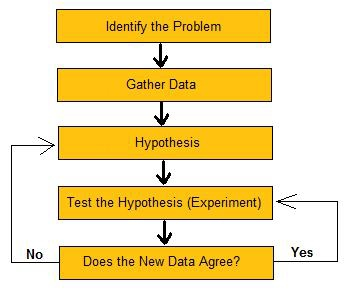
\includegraphics[width=11cm, height =9cm]{images/The_Scientific_Method.jpg}
\caption{Exemplo de metodologia em inglês.}
\legend{Fonte: Retirado da Wikimedia Commons.}
\label{fig:metodo}
\end{figure}

\subsection{Como fazer uma subseção}
Em seguida você vai ler 2 parágrafos de Lorem ipsum para encher linguíça.

\lipsum[2-4]
\subsection{Outra subseção}
Em seguida você vai ler 2 parágrafos de Lorem ipsum para encher linguíça.

\lipsum[2-4]
\section{Passo 2: Referências às seções do documento}\label{sec:refs}

Não adicione uma Seção \ref{sec:imagens} se você não tem uma Seção \ref{sec:refs} em seguida.  Em seguida você vai ler 2 parágrafos de Lorem ipsum para encher linguíça.

\lipsum[2-4]


